\section{Background}
\label{sec:background}

% I think this section should include an explanation of the types of cookies we looked for when searching for profiling cookies
Global cookies, such as DoubleClick's \texttt{id} cookie, have a globally unique value, \emph{i.e.,} its value remains the same across different visited websites in each \emph{session} (\textbf{NEEDS VERIFICATION: per session, or per lifetime}. 
Ad companies use these cookies to track user through their web and collect information about their browsing habits and personal preferences.

Local cookies, on the other hand, such as the Google Analytics \texttt{\_\_utma} cookie, have locally unique values.
This means that each unique domain that utilizes such a cookie to track an individual user will have a unique user identifier for the entire \emph{lifetime} of the cookie (\textbf{NEEDS VERIFICATION: per session, or per lifetime}.
These kinds of cookies are used by domains to keep track of their own users and their browsing habits pertaining to their website. 

\subsection{Cookies used by Google}
As Google cookies are one of the most pervasive cookies on the Internet we start by giving an overview of the different types of cookies that Google uses. They can be divided into the following categories:
\begin{itemize} \itemsep1pt \parskip0pt \parsep0pt

  \item Preferences
  \item Security
  \item Processes
  \item Advertising
  \item Session State
  \item Analytics

\end{itemize}

Preference cookies allow Google to keep track of user preferences in order to provide a more personalized browsing experience. Information stored include default language, user region, number of search results to display per page, text size and font and other preferences. Notably through the use of these cookies, Google does not require the user to be signed in to provide the targeted Google website. The PREF cookie is the most dominant cookie for storing user preferences. It also includes a timestamp of the most recent user preference change. This unique information can be used to pinpoint individual users due to the unlikelihood that two users have the same timestamp.

Security cookies are used to authenticate users and prevent fraudulent use of login credentials. They store the Google account ID and most recent sign-in time in an encrypted and signed string. Security cookie names end with SID, such as SID, HSID, SAPISID and APISID. The APISID cookie and SAPISID cookie both contain two encrypted strings, where the second string is \emph{unique across all Google websites and per cookie lifetime}. Therefore, despite the encryption, it is still possible to identify individual users and profile what Google services the user is visiting.

Process cookies support the display and function of more complex and dynamic websites. Google states that these cookies are necessary for the proper functioning of some websites. (\textbf{REFERENCE}) For example blooking an 'lbcs' cookie would prevent Google docs from opening documents correctly. BiscuitSpy does not include this cookie in its profiling.

Advertising cookies are used to determine which ads to display to the user and for tracking the user's ad clicking behavior through a complex network of publishers, advertisers and website operators. The most commonly seen advertising cookie is the 'id' cookie from the domain ad.doubleclick.net. The second field of the 'id' cookie contains several numbers that remain the same during multiple visits of the same website, but change their values either when the user has clicked on an advertisement on the website, or when the website displays a different ad. It can thus be inferred that the numbers encode the ads to display and whether the user has clicked on them.

Session state cookies collect information about how users interact with a website and keep information of the previous sessions of a website. Youtube session cookies for example store a list of most recent videos watched in that browser. Session state cookies are also used to measure the effectiveness of affiliate advertising. It is difficult to determine the exact names of session cookies and the meaning of their values, therefore BiscuitSpy currently does not leverage session cookies for user profiling.

Analytics cookies represent the largest group of Google cookies and are mainly used by BiscuitSpy to gather user profile information. While the previous cookies all belong to a Google domain, analytics cookies do not have that restriction and can be found on all websites that use Google Analytics (GA) and are stored under the current website's domain. The five main cookies set by GA are  \_utma,  \_utmb, \_utmc, \_utmv and \_utmz. 

\begin{figure}[h]
\centering
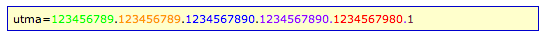
\includegraphics[scale=0.8]{./diagrams/utma.png}

\begin{tabular}{ | l | p{12cm} |}
    \hline
  Cookie Field & Description \\ \hline
Domain Hash & The first number is the domain hash. This is set by all cookies from this domain. \\ \hline
Visitor ID & The second number is a random "unique ID". \\ \hline
Initial visit & The third number is the unix time stamp for the initial visit and is set as soon as you enter the site. \\ \hline
Previous Session & The third number is the unix time stamp for the previous session. \\ \hline
Current Session & The fourth nubmer is the unix time stamp for the current session. \\ \hline
Session number & Contains the number of visits to this website since cookie creation. \\ \hline
 \end{tabular}

\caption{Google Analytics UTMA cookie}
\label{fig:utma}

\end{figure}

As an example, Figure \ref{fig:utma} shows the individual components of the \_utma cookie. The timestamp information of the initial, most recent and current visit in combination with the number of visits to the website allow for an accurate reconstruction of user's browsing behavior. 







